\documentclass{article}
\usepackage{tikzexlipsum}

%---------------------------------------------------------
\begin{document}
Usage: \verb|\usepackage{tikzexlipsum}|

%\tikzexmaxparcount\ items stored.\par

%\tikzexlipsum
%\tikzexlipsum[99-26]

\bigskip
Command \verb|\tikzexlipsum[27]| typesets the 27\textsuperscript{th} item:

\bigskip
\tikzexlipsum[27]
%\tikzexlipsum[\tikzexmaxparcount]%[f]


%\tikzexlipsum[21]
%\tikzexlipsumrr
%\tikzexlipsum[27]
%%\tikzexlipsum[27][f]
%%
%%\tikzexlipsumr[f]
%\tikzexlipsuma{5}\par
%\tikzexlipsumt{5}\par

%\tikzexlipsum[5-7][f]

\tikzexlipsumalist

%\tikzexlipsum[14][f]% no direct lua code inside a figure environment


\newpage
\fbox{Adding an item}

\begin{quotation}\noindent
\begin{verbatim}
\setuptikzexlipsum{
Attribution
}
{
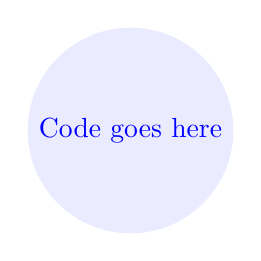
\begin{tikzpicture}
\node [circle, blue, fill=blue!8] (a) {Code goes here};
\end{tikzpicture}
}
\end{verbatim}
\end{quotation}

\setuptikzexlipsum{
Attribution
}
{
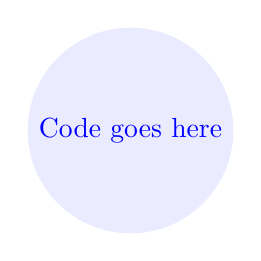
\begin{tikzpicture}
\node [circle, blue, fill=blue!8] (a) {Code goes here};
\end{tikzpicture}
}



\bigskip
\fbox{Calling the last-added item}

 (tikzexmaxparcount=\tikzexmaxparcount)


\begin{quotation}\noindent
\begin{verbatim}
\tikzexlipsum[\tikzexmaxparcount]
\end{verbatim}

\tikzexlipsum[\tikzexmaxparcount]

\end{quotation}



\newpage
\fbox{A random item}

with \verb|\tikzexlipsumr|

\tikzexlipsumr%



\end{document}